\documentclass[../main.tex]{subfiles}
\graphicspath{{\subfix{../images/}}} % Pfad zu den Bilddateien anpassen

\begin{document}

% Einleitung Abschnitt
\section{Einleitung}

% Textbeispiele für verschiedene Textstile
\textbf{Hello Bold world!} % Fettgedruckter Text
\textit{Hello Italic World!} % Kursiver Text

% Abbildung einfügen
\begin{figure}[h]
    \centering
    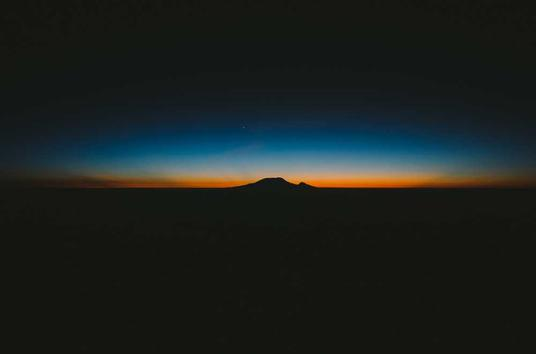
\includegraphics[width=3cm]{images/picsum lorem.jpg} % Pfad zur Abbildung
    \caption{Overleaf picsum lorem} % Beschriftung der Abbildung
    \label{fig:picsum_lorem} % Label für die Abbildung
\end{figure}

% Zitieren aus einem Text
Hier zitiere ich aus dem Text \autocite[10]{smith2018}. und schreibe dann weiter.\par % Beispiel für eine Zitierung


% % Verwendung von Abkürzungen
Hier benutzen wir Abkürzungen wie \gls{ml} und \gls{ai}.\\ % Beispiel für die Verwendung von Abkürzungen
Außerdem ist es jetzt hier \gls{ml} abgekürzt.\par % Wiederholte Verwendung der Abkürzung

% Acronyme werden in der Datei build/acronyms definiert

%Definition
\begin{definition}
Das ist eine Lustige definition.
\end{definition}

% Gesetzeszitat
Ein Beispieltext mit einem Gesetzeszitat \lawcite[§ 164 Absatz 1 Satz 1]{aktg1965}. % Beispiel für ein Gesetzeszitat

% Mehrere Seiten Zitierung
Hier ein zweites Zitat über mehrere Seiten \autocite[15-27]{johnson2020}. % Weitere Zitierung

\medskip

% Tabelle einfügen
\begin{table}[h]
    \centering
    \begin{tabular}{cc}
        Element1 & Element2\\
        Element3 & Element4\\
    \end{tabular}
    \caption{Beispiel-Tabelle} % Beschriftung der Tabelle
    \label{tab:example_table} % Label für die Tabelle
\end{table}

% Verweise auf Tabelle und Abbildung
In diesem Text referenziere ich auf die  \cref{tab:example_table} und danach auf das Bild \cref{fig:picsum_lorem}.

%AI Features
% Test der KI-Funktionen
\aikennzeichnung{ChatGPT 4.0}{Erkläre die Grundlagen des Marketings}{15.03.2024}

Dieser Absatz behandelt wichtige Konzepte.
\aiabschnitt{Claude 3.5}{Erstelle eine Marktanalyse für E-Commerce}{16.03.2024}

\aizusammenfassung{ChatGPT 4.0}{Fasse die wichtigsten Punkte zusammen}{17.03.2024}



\end{document}
